\documentclass[11pt,a4paper]{scrartcl}
%{{{ general stuff
\usepackage[a4paper,bindingoffset=0.2in,%
            left=1in,right=1in,top=1in,bottom=1in,%
            footskip=.25in]{geometry}
\usepackage[english]{babel}
\usepackage[utf8]{inputenc}
\usepackage[T1]{fontenc}
\usepackage{cite}
\usepackage[hidelinks]{hyperref}
\usepackage{float} % use H in figure placement
\pagenumbering{gobble}

%}}}
%{{{ graphics
\usepackage{graphicx} % Bilder
\usepackage{tikz, pgfplots}
\pgfplotsset{compat=1.14}
%}}}
%{{{ math
\usepackage{mathrsfs} % mathcal and mathscr
\usepackage{mathtools, amssymb, amsthm}
\usepackage{bm} % cool bold symbols
%}}}
% a todo command===============================================================
\usepackage[ruled]{algorithm2e}
\newcounter{todocounter}
\newcommand{\todo}[2][noisnotdefined]{
 \marginpar{\fcolorbox{black}{orange}{\footnotesize\textbf{todo}}
 \ifthenelse{\equal{#1}{noisnotdefined}}{}{\textcolor{black}{\newline\tiny #1}}}
 \textbf{\ifthenelse{\equal{#2}{.}}
   {\fcolorbox{orange}{white}{\textcolor{orange}{$\maltese$}}}{{\textcolor{orange}{#2}}}}
 \refstepcounter{todocounter}}

%===============================================================================

\date{}
\title{todo: think about good title}
\author{Felix Bartel and D\'avid Kerekes}


\begin{document}

\maketitle

\section{Introduction}



Undoubtedly, the neural network architecture has been the star of the machine learning resurgence of the past few years. It's provable quality of being an universal function approximator makes it a sensible choice for various applications from control to . The main algorithm used for training, backpropagation however is subject to an array of criticism from various authors \cite{some_papers_about_backprop}, and there are various attempts at improving or replacing it \cite{that_paper_where_ga_beats_backprop}.
\todo{Add a sentence of context for \cite{Sims94evolving3d} and \cite{Garis90geneticprogramming}}

In this work we explore some properties of neuroevolution, the technique of applying a genetic algorithm to a neural network \cite{Garis90geneticprogramming} \cite{Sims94evolving3d}.
A big advantage of this scheme is that for a series of different inputs a single scalar indicator of performance is sufficient in order to optimize a neural network for a certain task.
This can for instance be given by the outcome of a game.
Our game of choice is Blobby Volley 2 which is an open source, simple two-dimensional volleyball game written in C++ with lua support. See Figure \ref{fig:screenshot}.

\begin{figure}[H]
\center
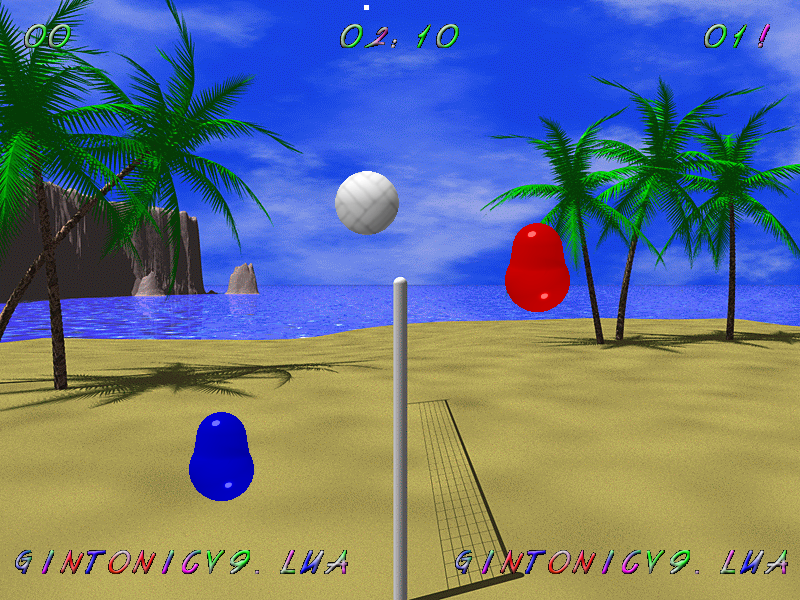
\includegraphics[width=0.4\textwidth]{img/screenshot.png}
\caption{Screenshot of the game.}
\label{fig:screenshot}
\end{figure}

\section{Training environment}

A scene from the game could be described by the $x$- and $y$-coordinates of the players and the ball, their corresponding velocities and the current number of ball contacts.
These arguments or a subset of them can then be used as input for the neural network.
The output should correspond to the possible movement options of the player, which consists of going right, going left, or jumping.
Assuming the layers of the neural network have $n_1,\dots,n_L$ nodes we then have to optimize \(N = \sum_{l=1}^{L-1} (n_l+1) \, n_{l+1}\) number of variables.

The game comes bundled with a number of bots with different styles, that are designed to pose a challenge to a wide range of human opponents. In order to define a clean ranking between them, we recorded the score of all possible lineups. The results can be seen in table no. \ref{tab:bot_vs_bot}.
\todo{explain the table}

\begin{figure}[H]
\begin{tabular}{c|ccccccc}
vs. &
\texttt{Axji-0-2} &
\texttt{COM\_11} &
\texttt{GintonicV9} &
\texttt{Hypo14} &
\texttt{reduced} &
\texttt{Union} &
\texttt{trainer} \\
\hline
\texttt{Axji-0-2} & - & 0 & 0 & 4 & 0 & 0 & 10 \\
\texttt{COM\_11} & 21 & - & 9 & 19 & 6 & 16 & 20 \\
\texttt{GintonicV9} & 21 & 12 & - & 19 & 6 & 16 & 20 \\
\texttt{Hypo14} & 17 & 2 & 2 & - & 2 & 5 & 15 \\
\texttt{reduced} & 21 & 19 & 15 & 19 & - & 19 & 21 \\
\texttt{Union} & 21 & 14 & 5 & 16 & 2 & - & 20 \\
\texttt{trainer} & 11 & 0 & 1 & 6 & 0 & 1 & -
\end{tabular}
\label{tab:bot_vs_bot}
\caption{Scores of bots competing against each other}
\end{figure}

We implemented our own bot to act as an initial trainer \texttt{trainer} for the network.
This trainer is easier to defeat.
We made a copy of each bot where it gives up after a certain amount of touches with the ball, such that normal gameplay will be rewarded.
The simplification gives the evolutionary algorithm the opportunity to start optimizing the neural network in a valid direction, without introducing additional factors to the fitness score.

\section{Implementation}
The genotype-representation of the network is accomplished through python objects. This allows a straightforward implementation of a wide variety of genetic operators. Since our algorithm is constrained overwhelmingly by evaluation time, these inefficient but easy to modify structures do not impact performance.
As the evaluation of the population is time-consuming, we do this in a thread-parallel fashion, allowing us to exploit multiple high core-count machines at our disposal.

\section{Standard genetic algorithm}

\subsection{Network architecture}

For the whole experiment, we fixed the size of the neural network to $6$ input nodes, one hidden layer with $7$ nodes and $2$ output nodes. As can be seen later, this proved sufficient for a surprisingly high performance for the network. The input nodes got fed with the x and y positions of the player, it's relative position compared to the ball, and the velocity vector of the ball.
The output nodes consisted of two neurons with tanh activations, one responsible for going left or right in the next timestep (if the output was below or above of threshold values $t_l = 0.49, t_r = 0.51$) and the other for jumping (when above threshold $t_j = 0.7$).

\subsection{Scheme}
The algorithm worked with a population size of 100, with 150 offspring after crossover. Our survivor selection strategy was elitism, selecting from the pool of children plus the 10 best parents from the last generation.

The fitness function was the normalized point difference after $21$ serves.

\subsection{Mutation}
Mutation is accomplished by adding Gaussian noise to a subset of all weights and biases. \todo{Default values, rate of change}

\subsection{Crossover}
As crossover we randomly mixed the nodes with belonging weights and biases of two networks and chose the parents via the fitness proportional roulette wheel selection. \todo{cite roulett wheel sel.}


\subsection{Numerical tests}

\begin{figure}[H]
\center
\begin{tabular}{ccc}
\texttt{reduced} & \texttt{com\_11} & \texttt{gintonicV9} \\
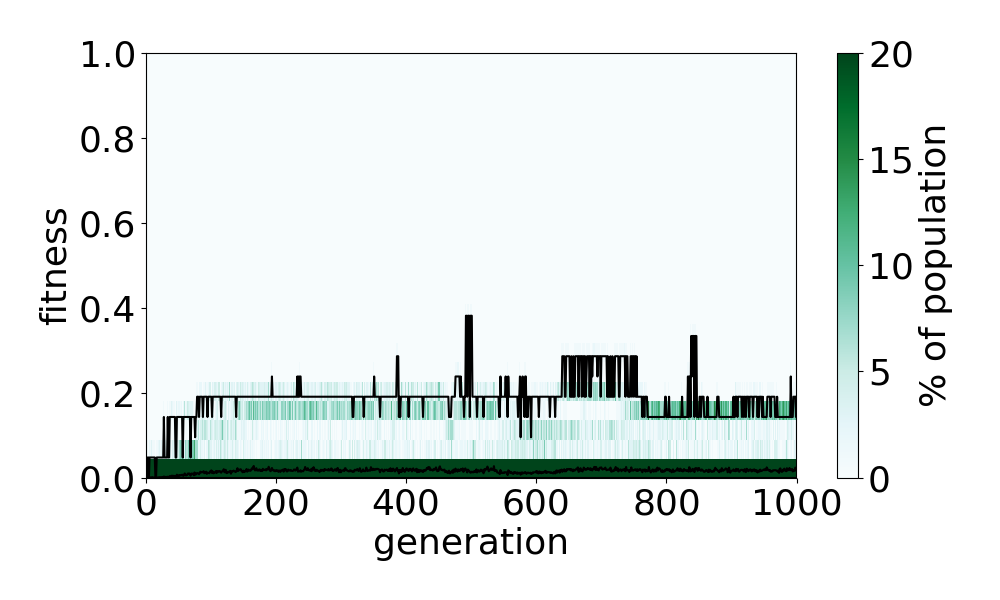
\includegraphics[width=0.3\textwidth]{img/standard_reduced.png} &
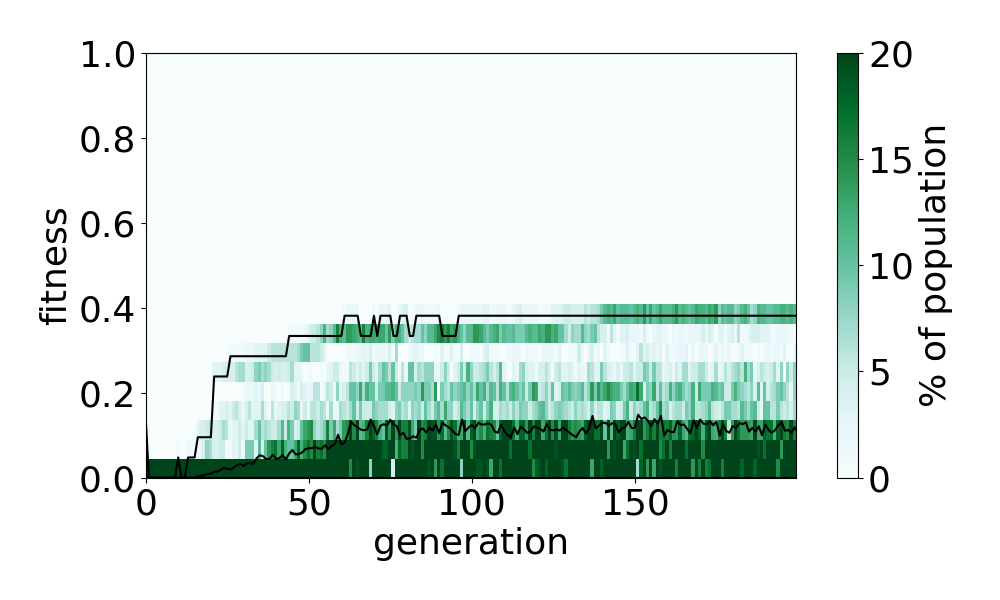
\includegraphics[width=0.3\textwidth]{img/standard_com_11.png} &
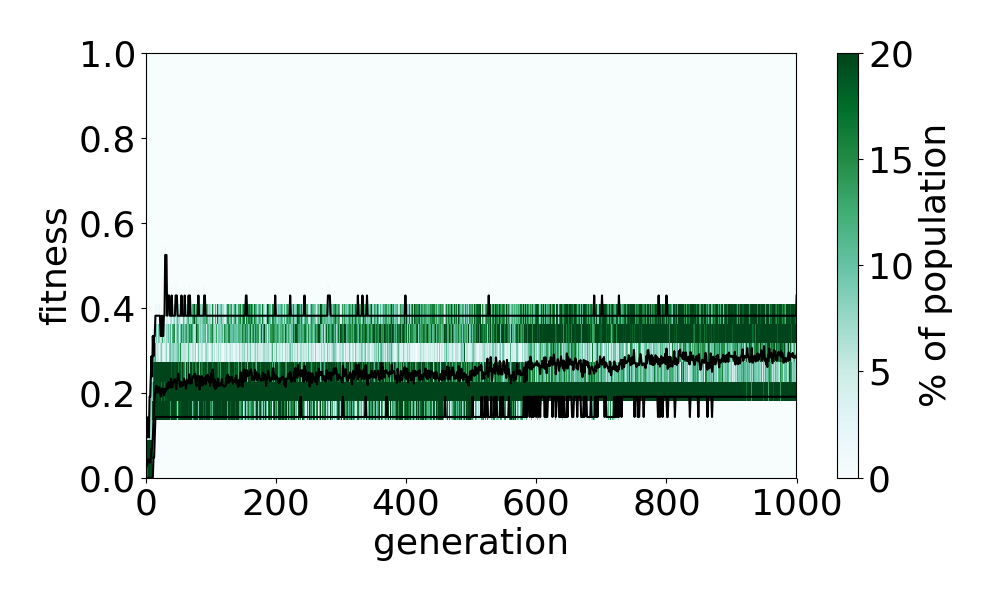
\includegraphics[width=0.3\textwidth]{img/standard_gintonicV9.png} \\
\texttt{hyp014} & \texttt{Union} & \texttt{trainer} \\
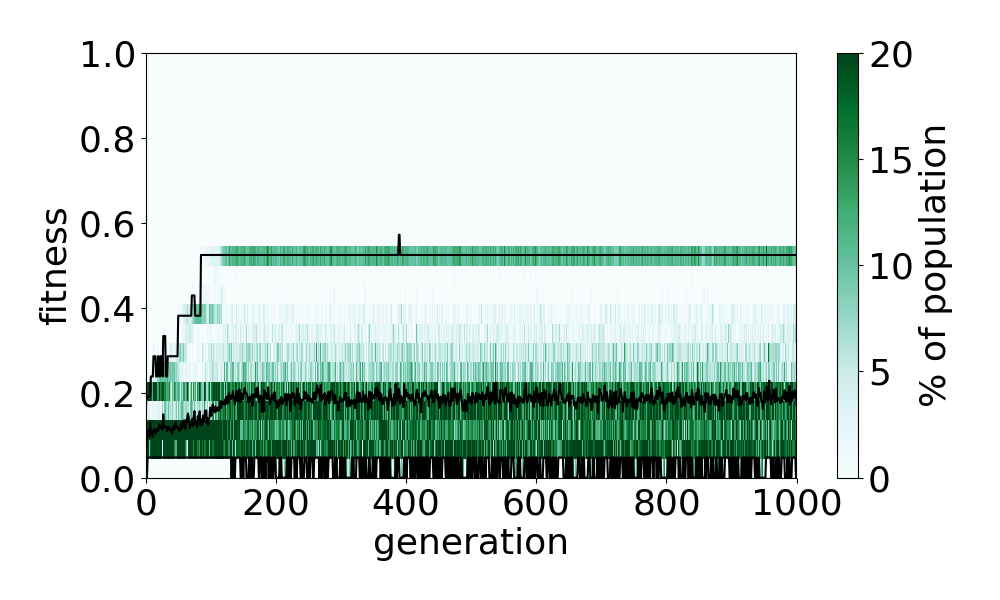
\includegraphics[width=0.3\textwidth]{img/standard_hyp014.png} &
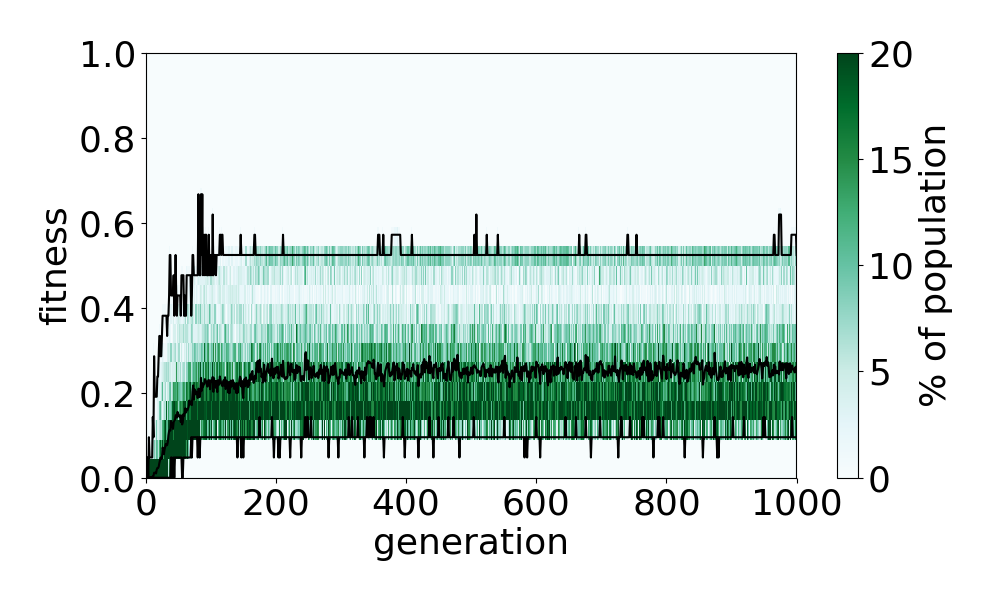
\includegraphics[width=0.3\textwidth]{img/standard_Union.png} &
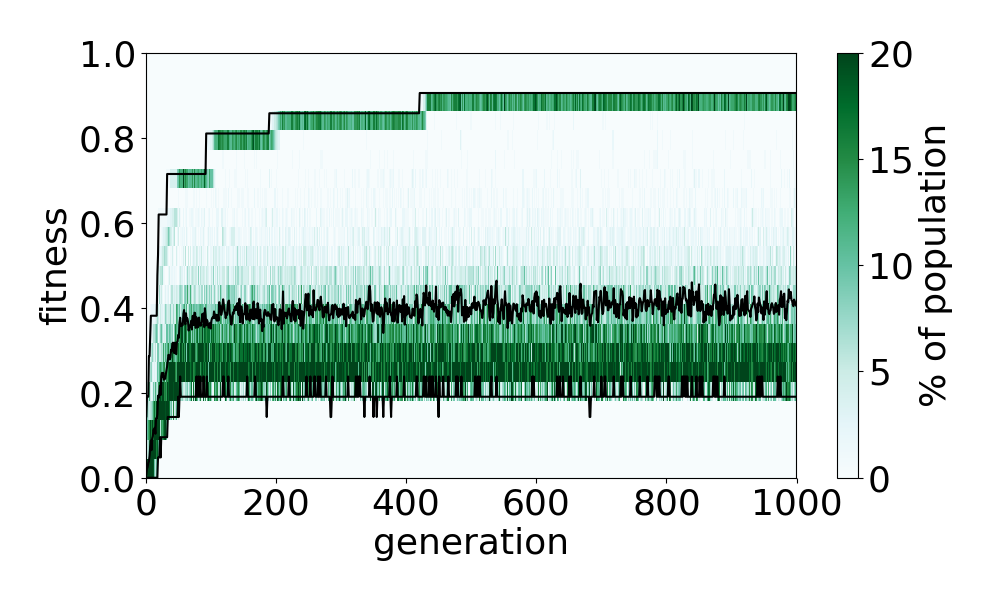
\includegraphics[width=0.3\textwidth]{img/standard_trainer.png}
\end{tabular}
\caption{Fitness density with indicated minimum, average and maximum while training against different bots. \todo{is this true?}}
\label{fig:standard}
\end{figure}

\begin{figure}[H]
\center
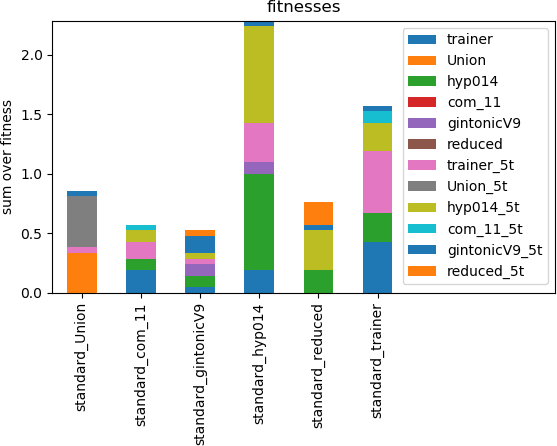
\includegraphics[width=0.4\textwidth]{img/standard.png}
\caption{trained bots against all other}
\label{fig:standard}
\end{figure}

\todo{coclusion: bots too hard we therefore reward gameplay by the *\_5t bots}

\todo{introduce the goal of an overall good bot and explain the plot along the way (added fitnesses (score of 12 would mean winneing every point against every bot))}


\begin{figure}[H]
\center
\begin{tabular}{ccc}
\texttt{reduced\_5t} & \texttt{com\_11\_5t} & \texttt{gintonicV9\_5t} \\
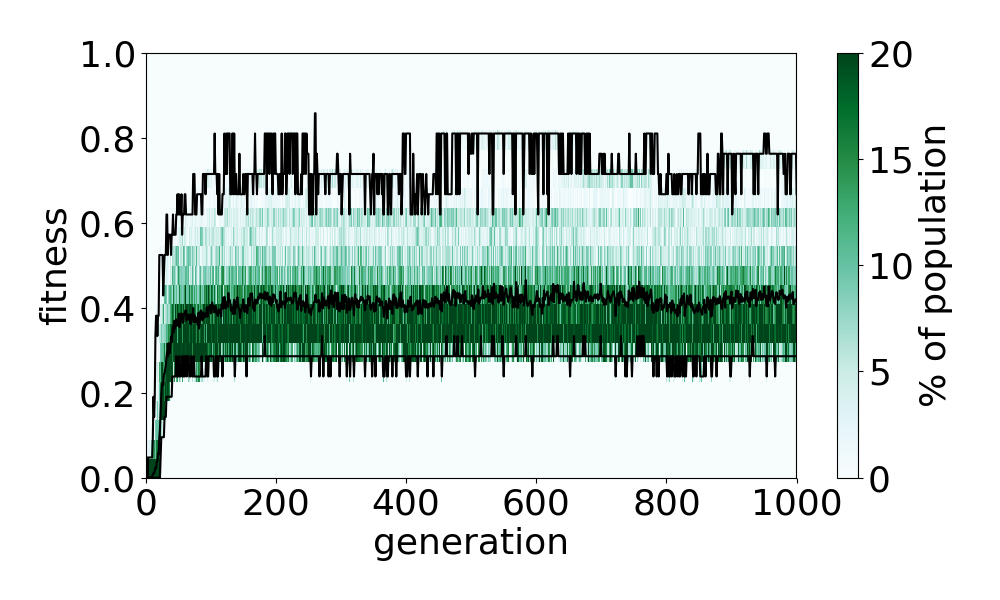
\includegraphics[width=0.3\textwidth]{img/standard_reduced_5t.png} &
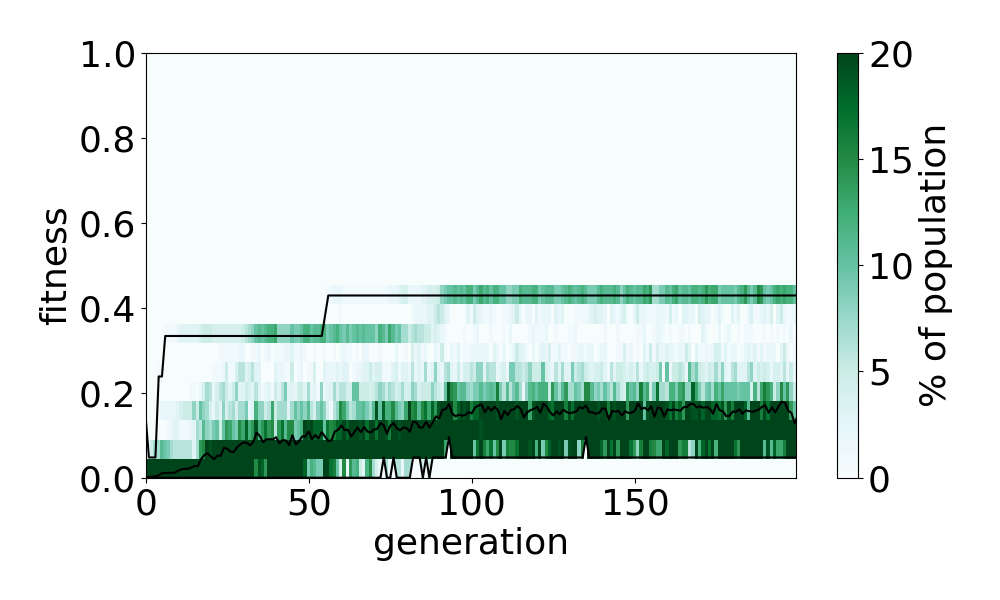
\includegraphics[width=0.3\textwidth]{img/standard_com_11_5t.png} &
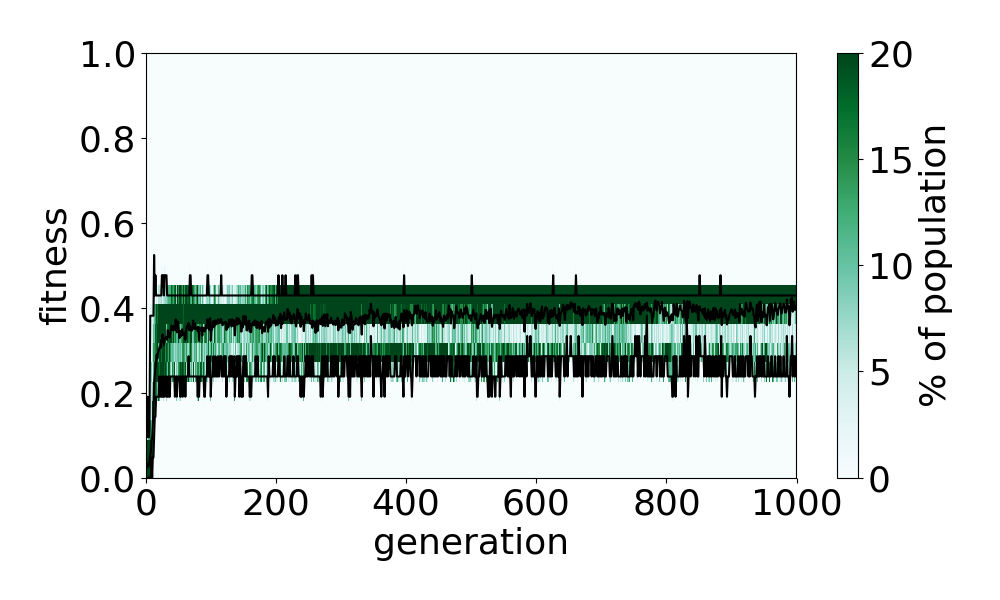
\includegraphics[width=0.3\textwidth]{img/standard_gintonicV9_5t.png} \\
\texttt{hyp014\_5t} & \texttt{Union\_5t} & \texttt{trainer\_5t} \\
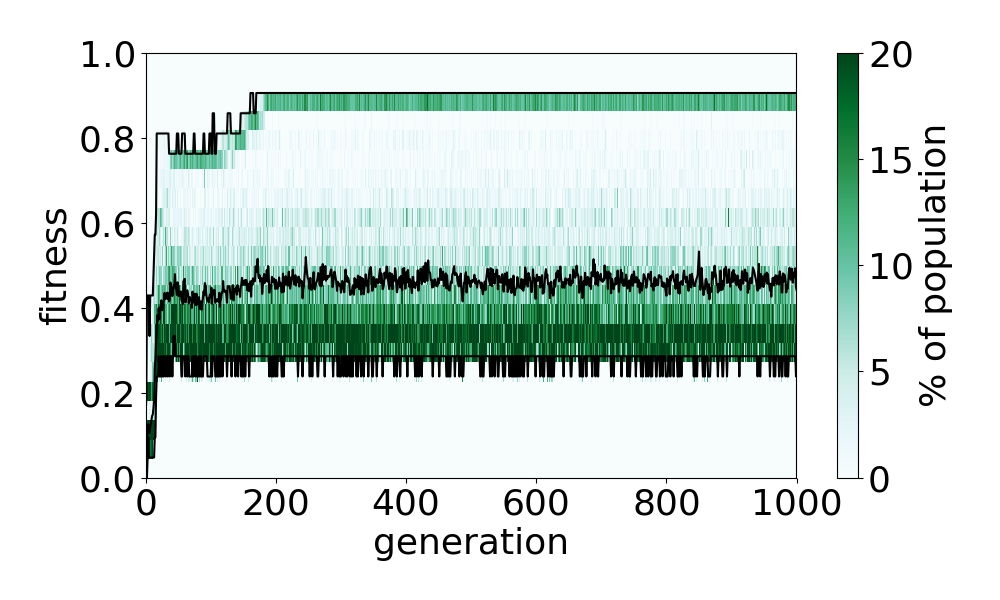
\includegraphics[width=0.3\textwidth]{img/standard_hyp014_5t.png} &
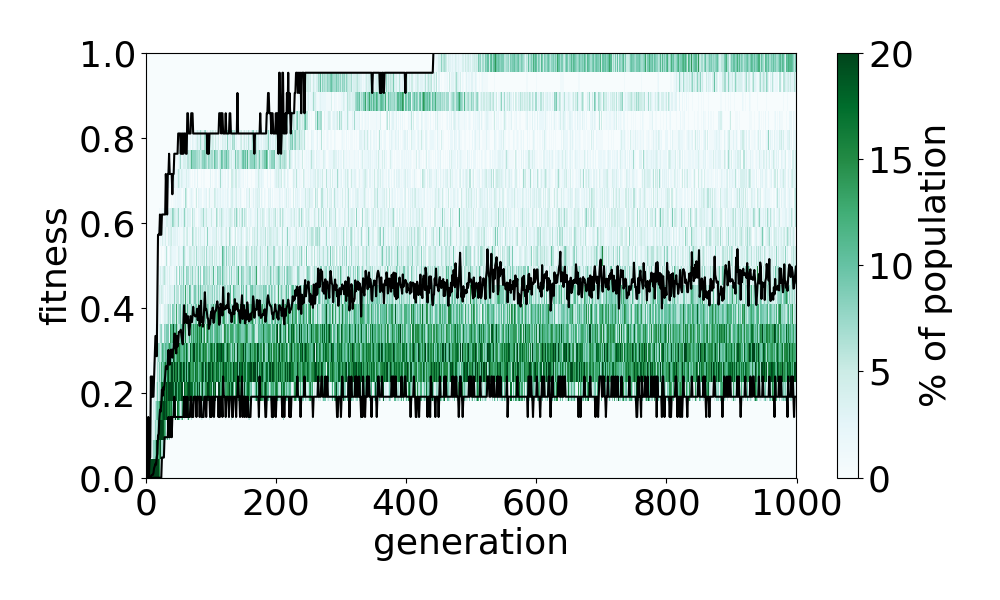
\includegraphics[width=0.3\textwidth]{img/standard_Union_5t.png} &
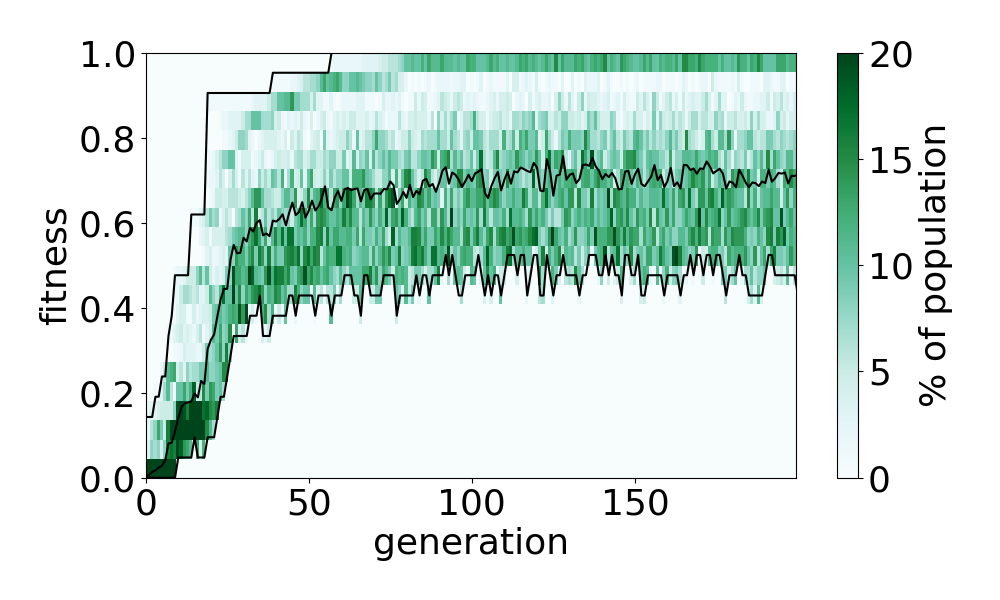
\includegraphics[width=0.3\textwidth]{img/standard_trainer_5t.png}
\end{tabular}
\caption{Fitness density with indicated minimum, average and maximum.}
\label{fig:standard_5t}
\end{figure}

\begin{figure}[H]
\center
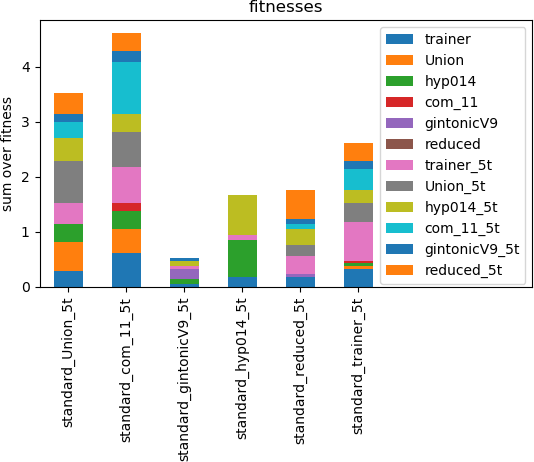
\includegraphics[width=0.4\textwidth]{img/standard_5t.png}
\caption{Trained bots against all other}
\label{fig:standard_5t_aa}
\end{figure}

\todo{conclusion: better, and not only for 5t bots (algorithm has something to grab on)}

\todo{overall: not very pretty graphs -> need self adaption}

\section{Self adapt 1}

\todo{explain what we are doing}

\subsection{Numerical tests}

\begin{figure}[H]
\center
\begin{tabular}{ccc}
\texttt{reduced} & \texttt{com\_11} & \texttt{gintonicV9} \\
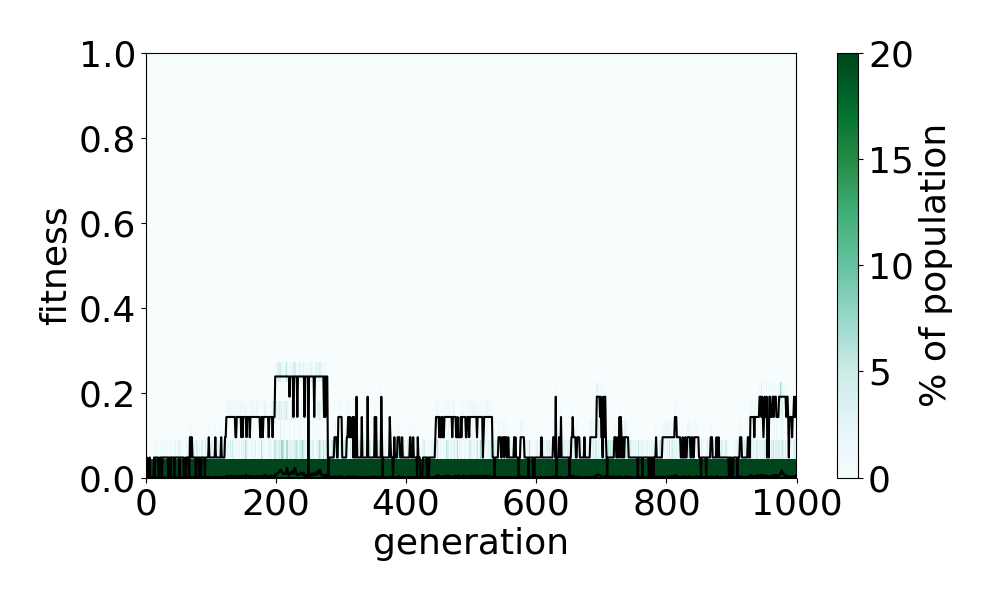
\includegraphics[width=0.3\textwidth]{img/self_adapt_1_reduced.png} &
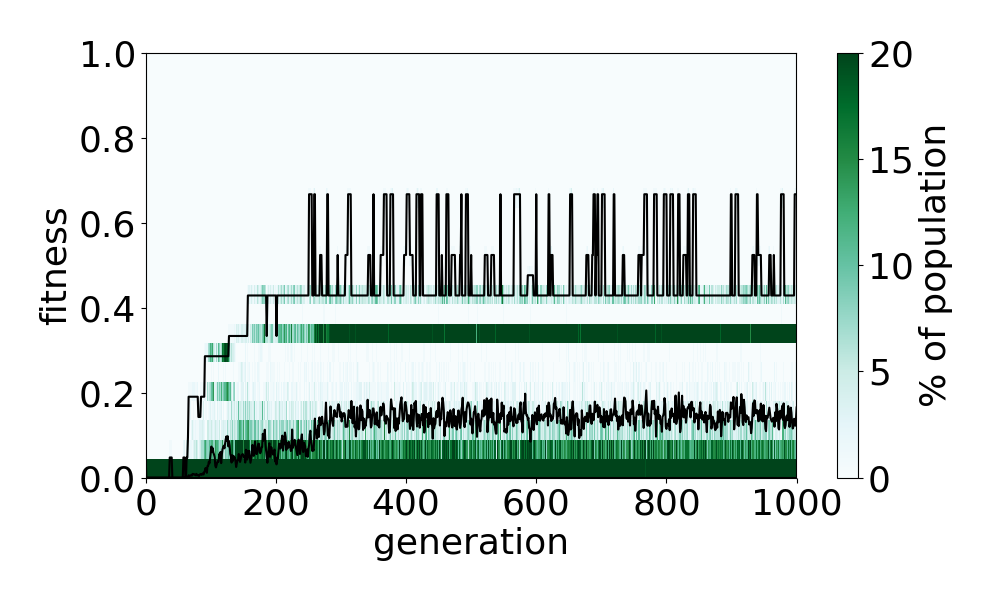
\includegraphics[width=0.3\textwidth]{img/self_adapt_1_com_11.png} &
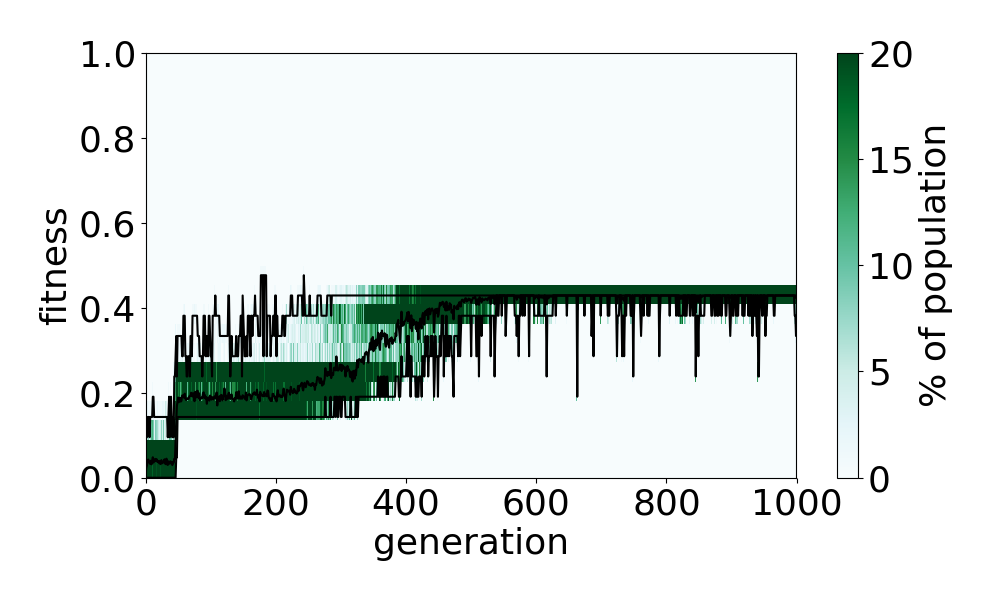
\includegraphics[width=0.3\textwidth]{img/self_adapt_1_gintonicV9.png} \\
\texttt{hyp014} & \texttt{Union} & \texttt{trainer} \\
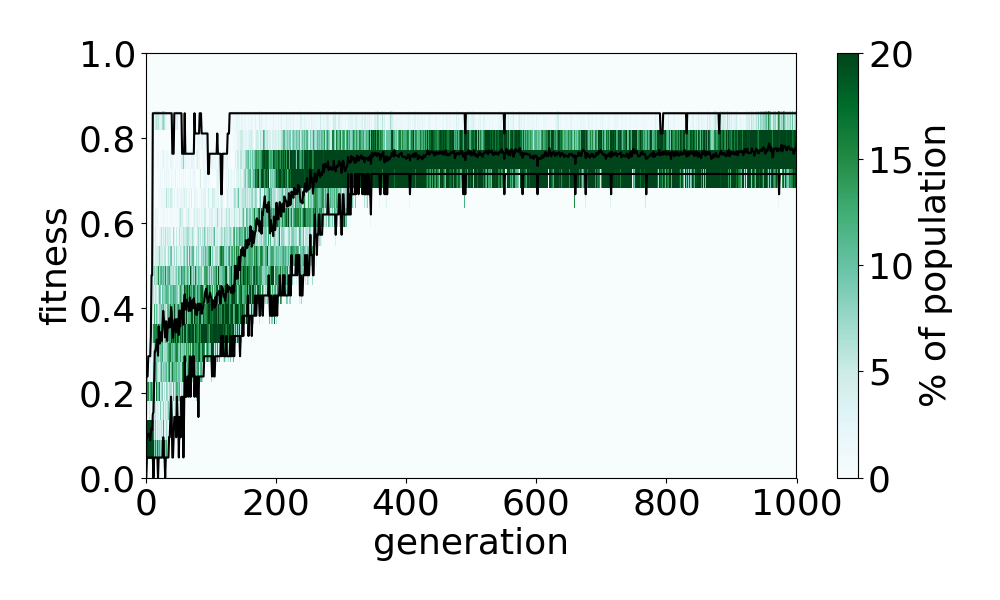
\includegraphics[width=0.3\textwidth]{img/self_adapt_1_hyp014.png} &
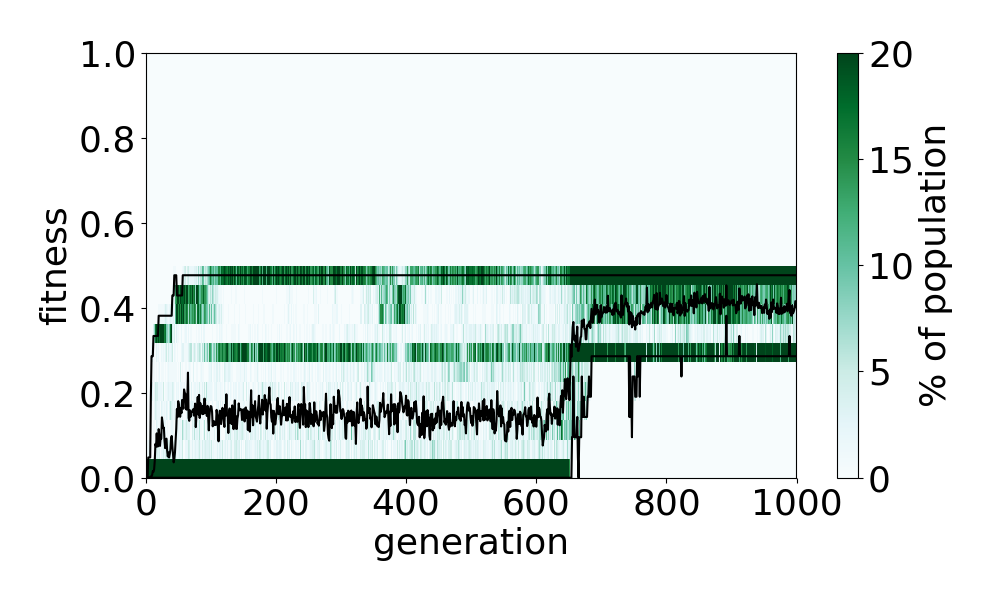
\includegraphics[width=0.3\textwidth]{img/self_adapt_1_Union.png} &
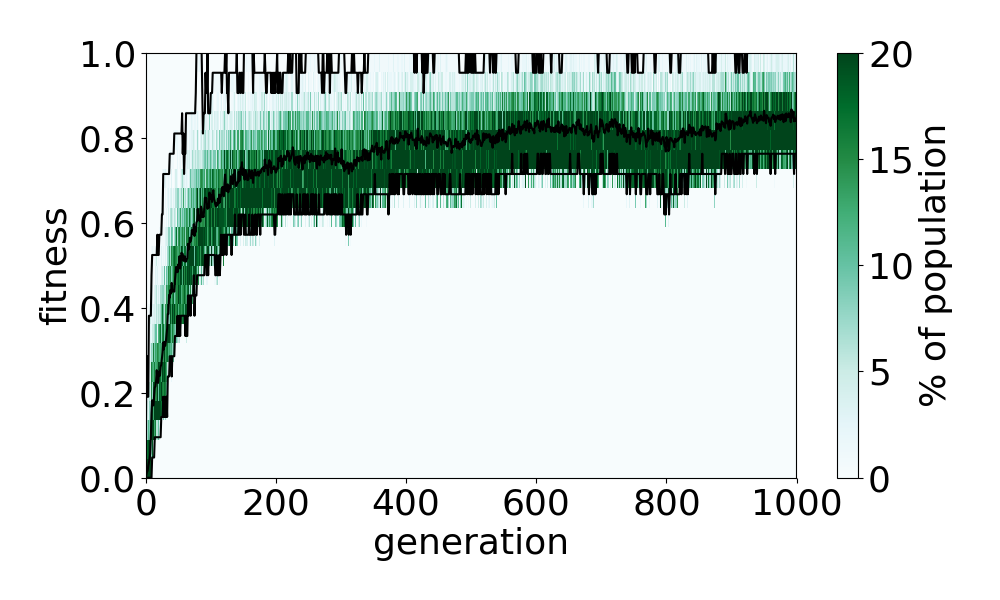
\includegraphics[width=0.3\textwidth]{img/self_adapt_1_trainer.png}
\end{tabular}
\caption{Fitness density with indicated minimum, average and maximum.}
\label{fig:self_adapt_1}
\end{figure}

\begin{figure}[H]
\center
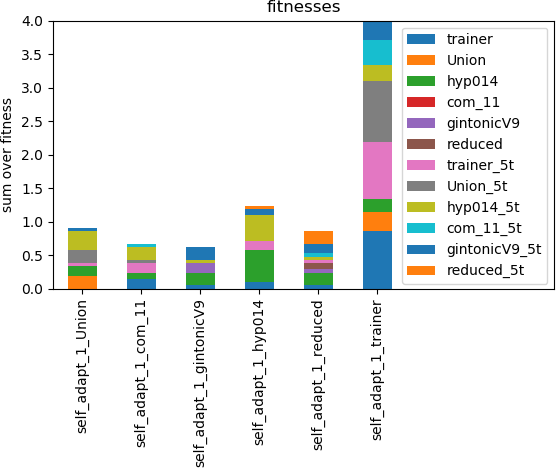
\includegraphics[width=0.4\textwidth]{img/self_adapt_1.png}
\caption{trained bots against all other}
\label{fig:self_adapt_1_aa}
\end{figure}

\todo{we can see that the algorithm is converging}
\todo{because trainer is beatable, the nn has something to grab on and performs way better thatn the others}

\begin{figure}[H]
\center
\begin{tabular}{ccc}
\texttt{reduced\_5t} & \texttt{com\_11\_5t} & \texttt{gintonicV9\_5t} \\
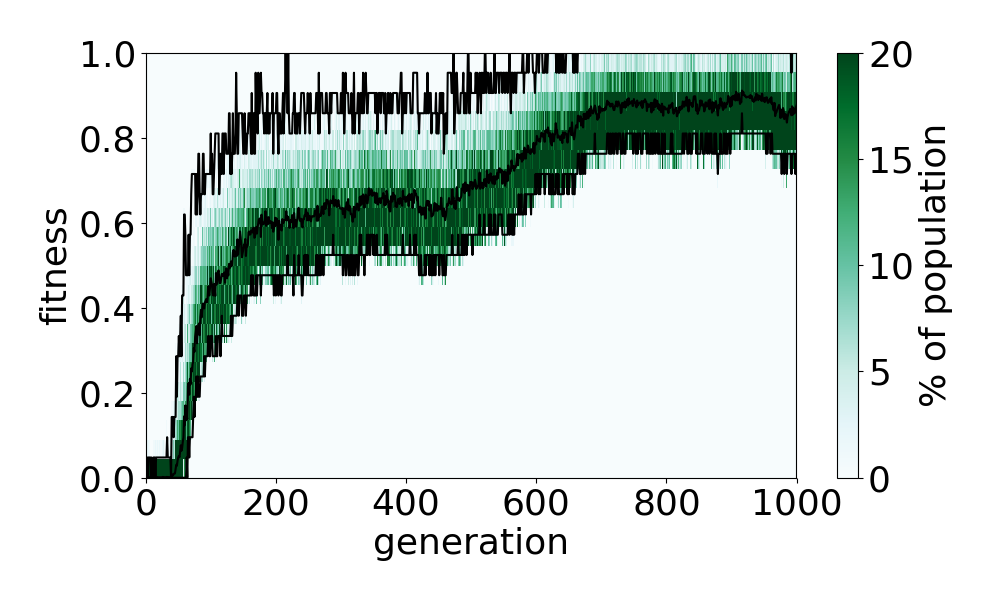
\includegraphics[width=0.3\textwidth]{img/self_adapt_1_reduced_5t.png} &
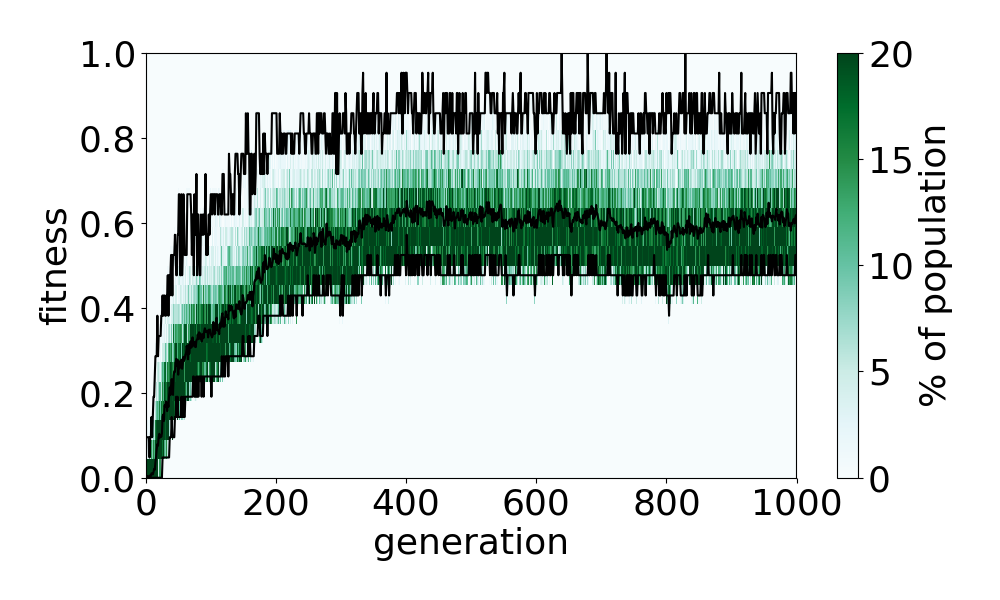
\includegraphics[width=0.3\textwidth]{img/self_adapt_1_com_11_5t.png} &
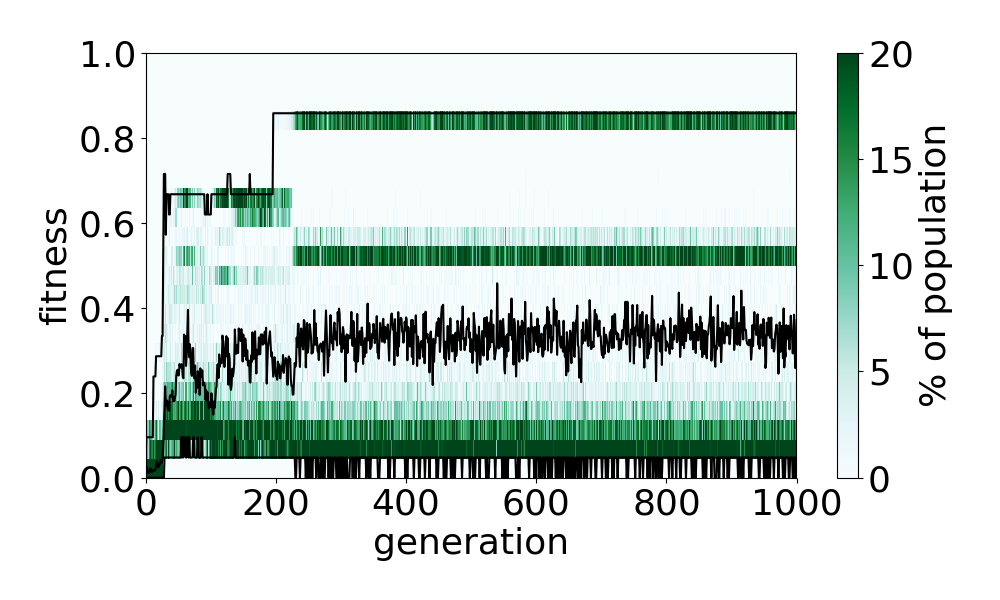
\includegraphics[width=0.3\textwidth]{img/self_adapt_1_gintonicV9_5t.png} \\
\texttt{hyp014\_5t} & \texttt{Union\_5t} & \texttt{trainer\_5t} \\
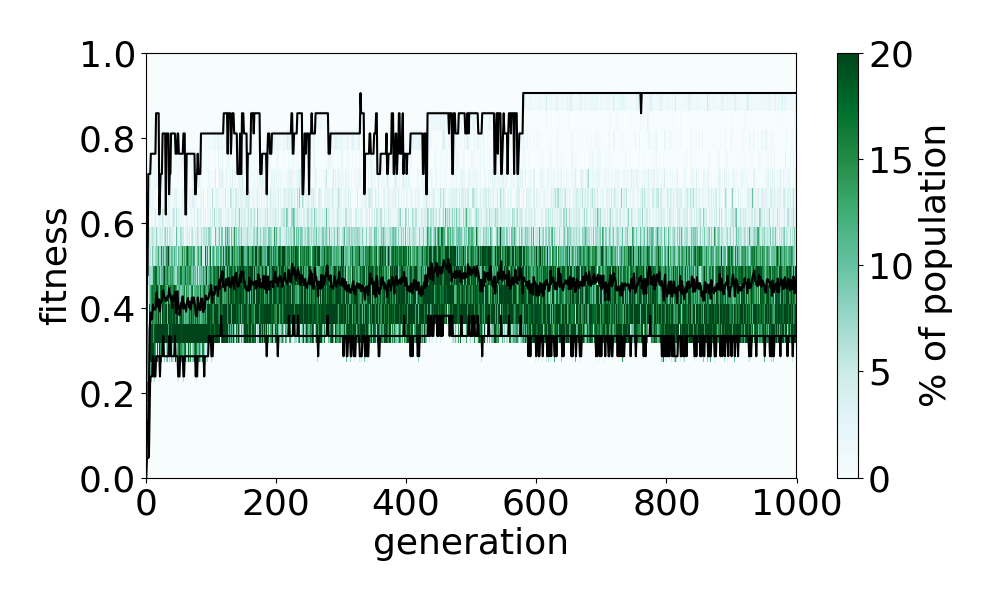
\includegraphics[width=0.3\textwidth]{img/self_adapt_1_hyp014_5t.png} &
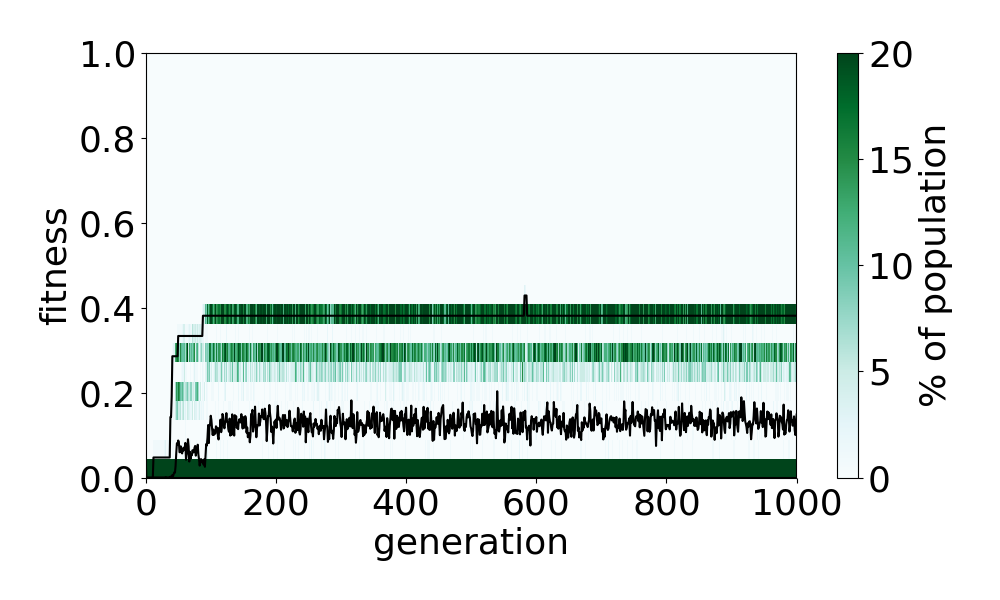
\includegraphics[width=0.3\textwidth]{img/self_adapt_1_Union_5t.png} &
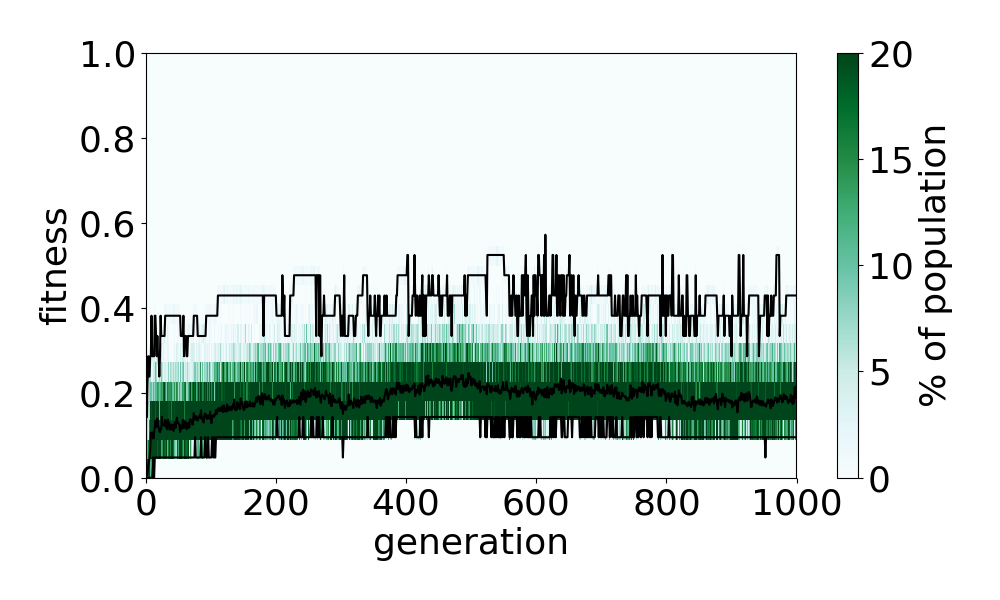
\includegraphics[width=0.3\textwidth]{img/self_adapt_1_trainer_5t.png}
\end{tabular}
\caption{Fitness density with indicated minimum, average and maximum.}
\label{fig:self_adapt_1_5t}
\end{figure}

\begin{figure}[H]
\center
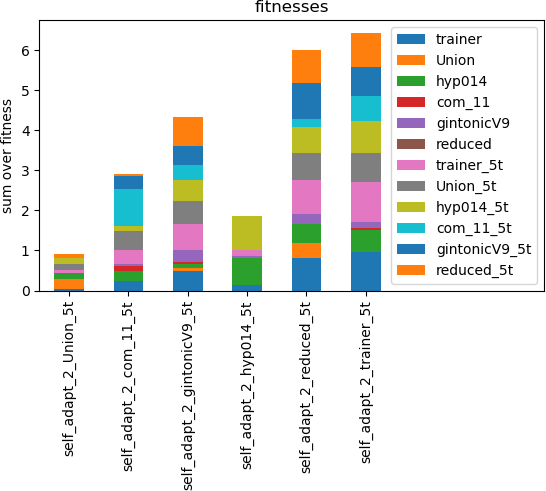
\includegraphics[width=0.4\textwidth]{img/self_adapt_2_5t.png}
\caption{trained bots against all other}
\label{fig:self_adapt_2_5t_aa}
\end{figure}

\todo{now it's pretty}
\todo{trainer\_5t bad because it is very easy to beat and therefore we can get loast in a local optimum real quick}

\section{Self adapt 2}


\subsection{Numerical tests}

\begin{figure}[H]
\center
\begin{tabular}{ccc}
\texttt{reduced} & \texttt{com\_11} & \texttt{gintonicV9} \\
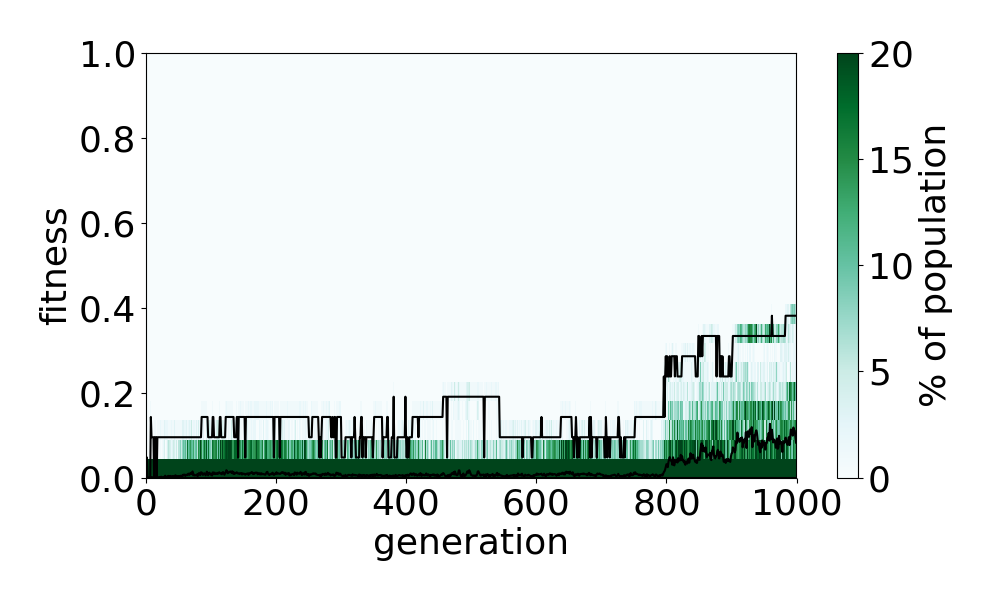
\includegraphics[width=0.3\textwidth]{img/self_adapt_2_reduced.png} &
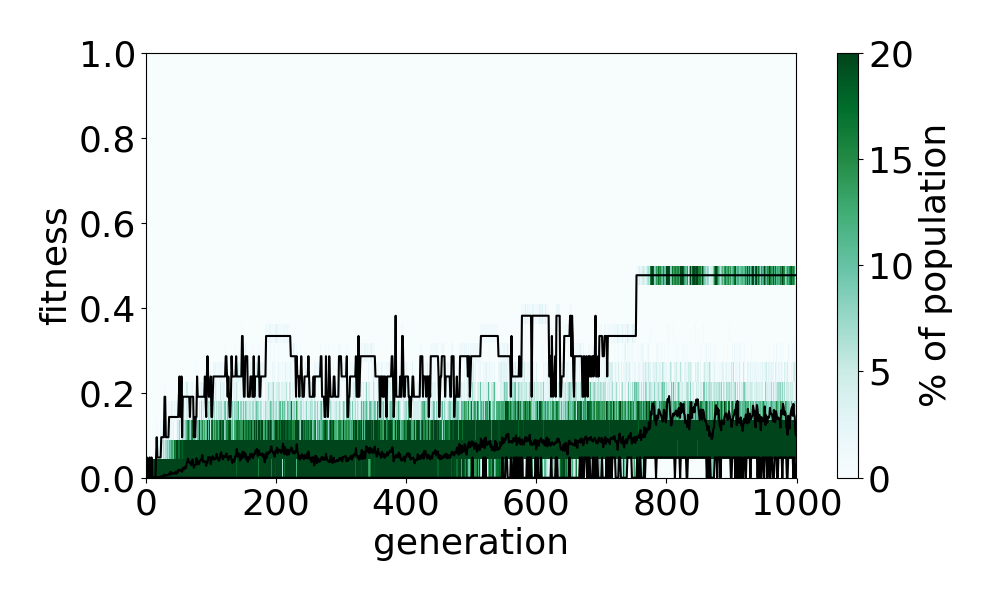
\includegraphics[width=0.3\textwidth]{img/self_adapt_2_com_11.png} &
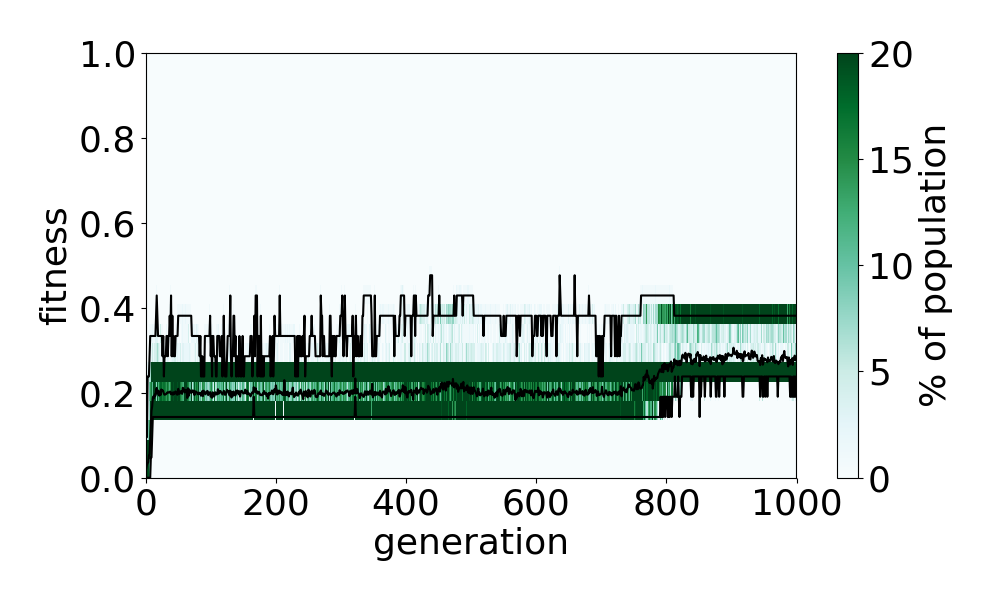
\includegraphics[width=0.3\textwidth]{img/self_adapt_2_gintonicV9.png} \\
\texttt{hyp014} & \texttt{Union} & \texttt{trainer} \\
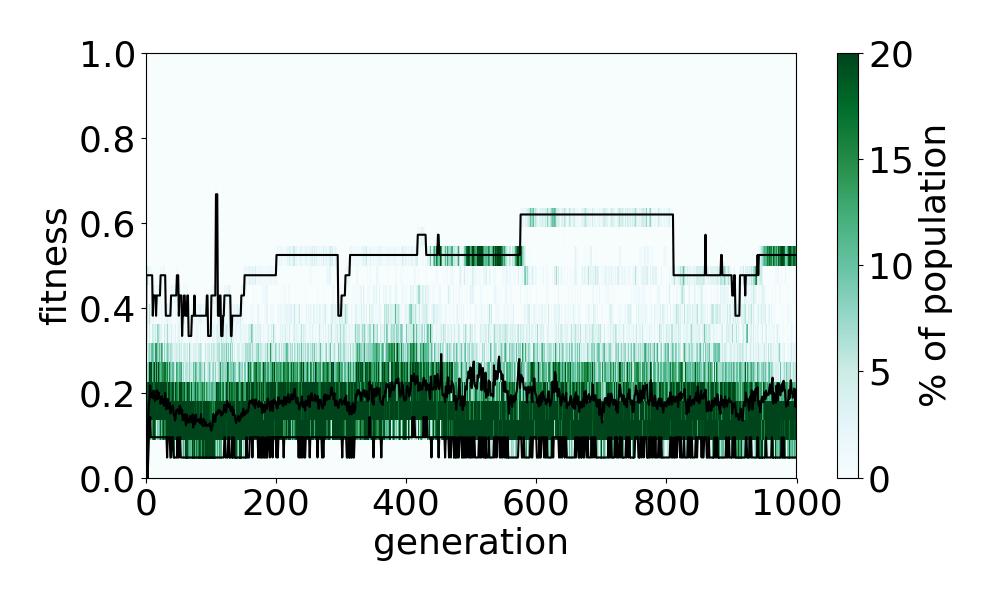
\includegraphics[width=0.3\textwidth]{img/self_adapt_2_hyp014.png} &
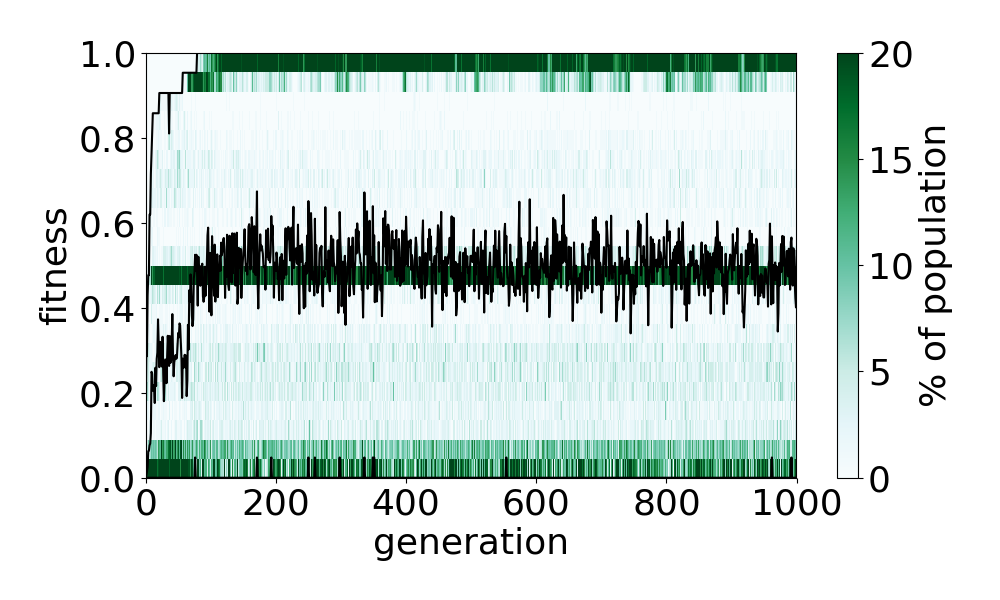
\includegraphics[width=0.3\textwidth]{img/self_adapt_2_Union.png} &
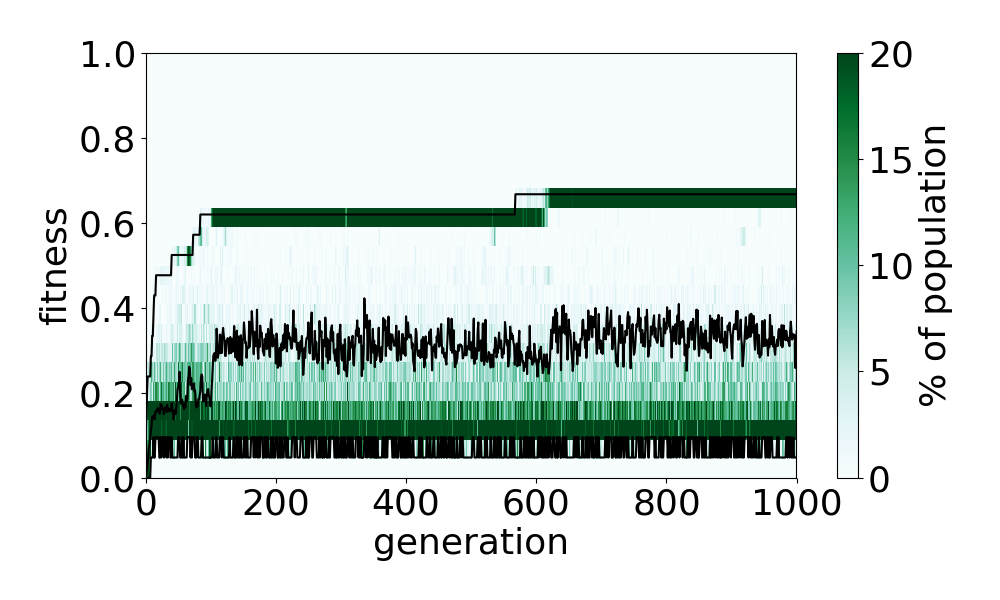
\includegraphics[width=0.3\textwidth]{img/self_adapt_2_trainer.png}
\end{tabular}
\caption{Fitness density with indicated minimum, average and maximum.}
\label{fig:self_adapt_2}
\end{figure}

\begin{figure}[H]
\center
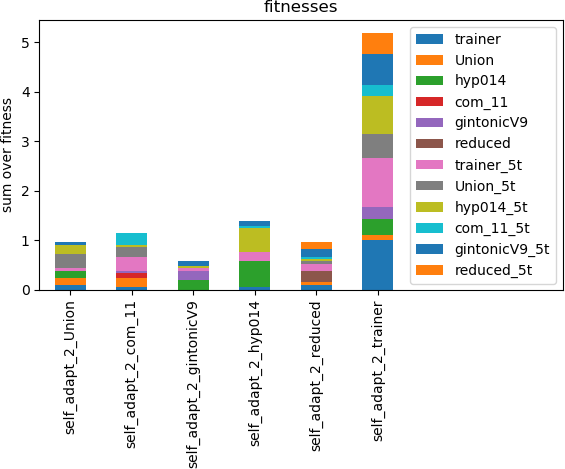
\includegraphics[width=0.4\textwidth]{img/self_adapt_2.png}
\caption{trained bots against all other}
\label{fig:self_adapt_2_aa}
\end{figure}

\todo{similar to section before without 5t}

\begin{figure}[H]
\center
\begin{tabular}{ccc}
\texttt{reduced\_5t} & \texttt{com\_11\_5t} & \texttt{gintonicV9\_5t} \\
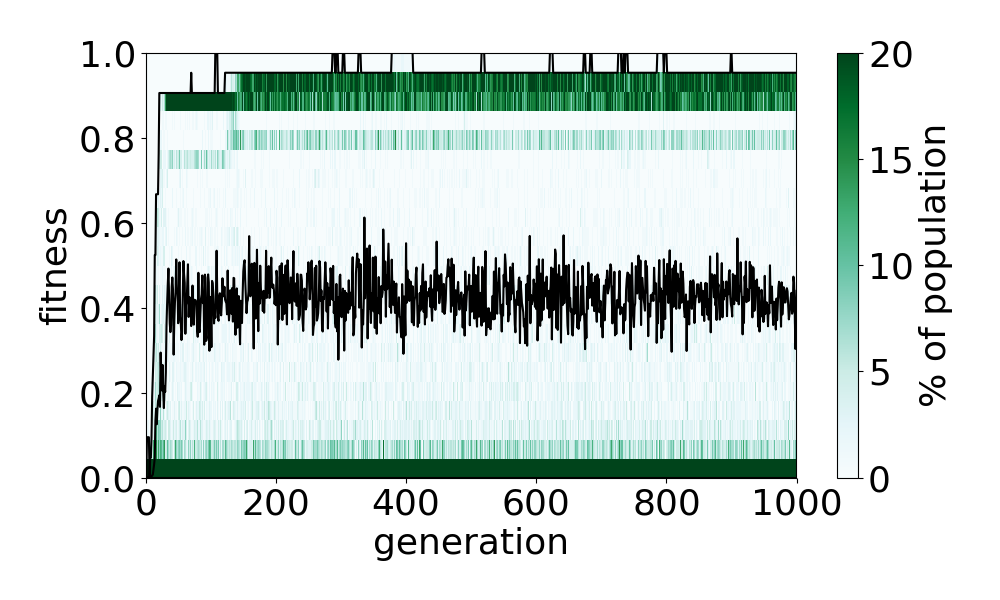
\includegraphics[width=0.3\textwidth]{img/self_adapt_2_reduced_5t.png} &
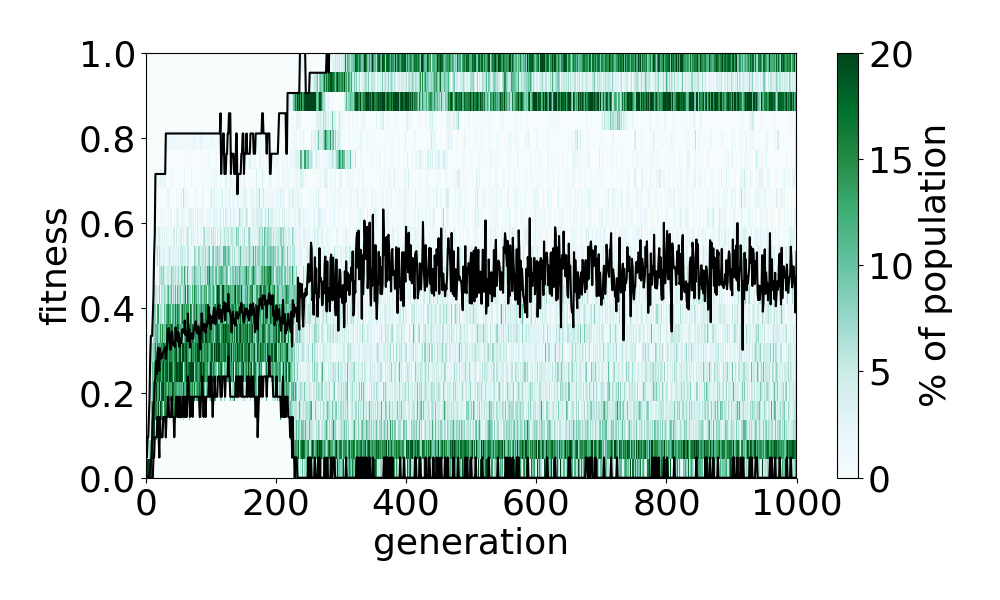
\includegraphics[width=0.3\textwidth]{img/self_adapt_2_com_11_5t.png} &
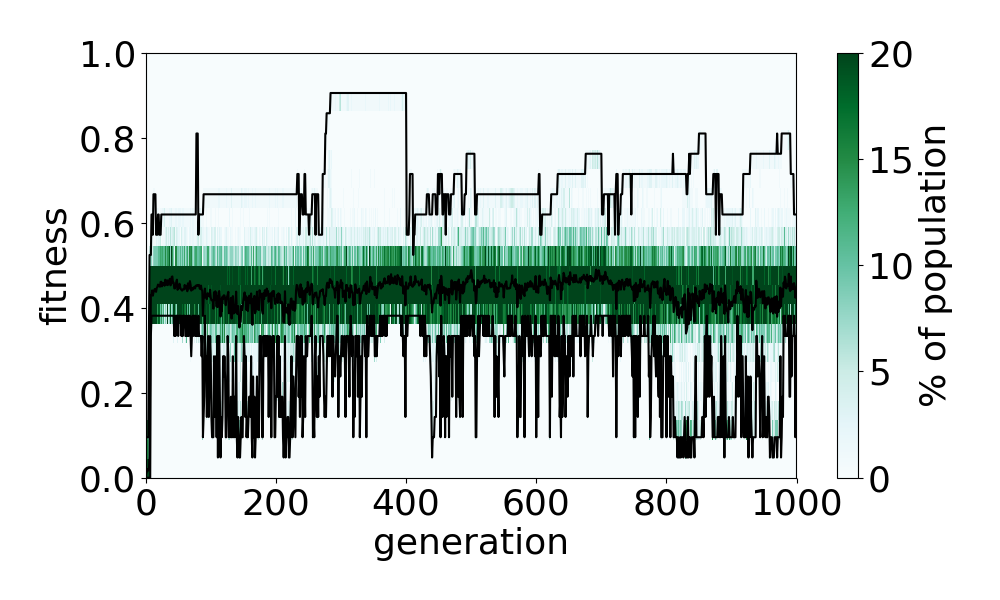
\includegraphics[width=0.3\textwidth]{img/self_adapt_2_gintonicV9_5t.png} \\
\texttt{hyp014\_5t} & \texttt{Union\_5t} & \texttt{trainer\_5t} \\
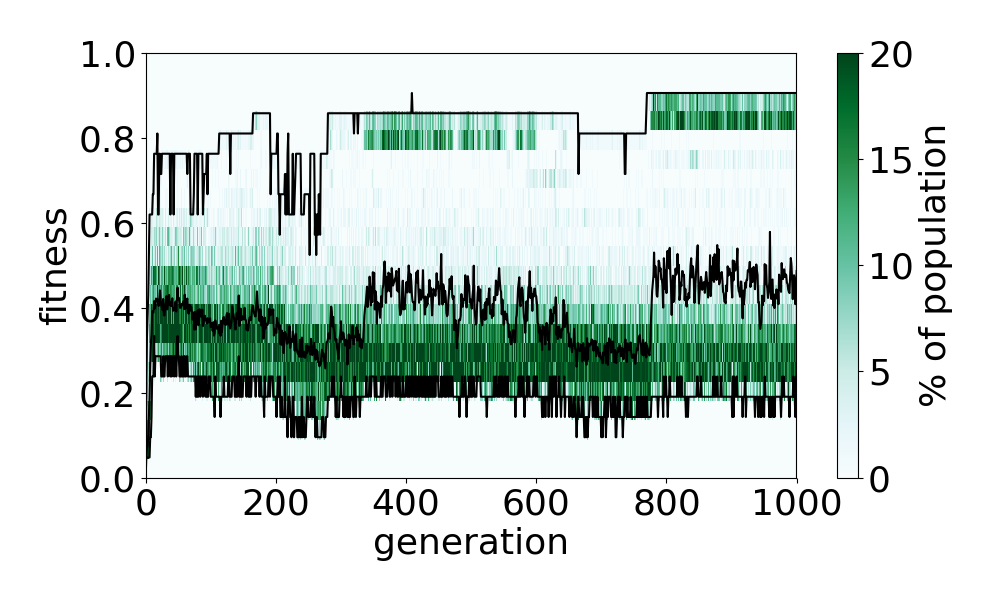
\includegraphics[width=0.3\textwidth]{img/self_adapt_2_hyp014_5t.png} &
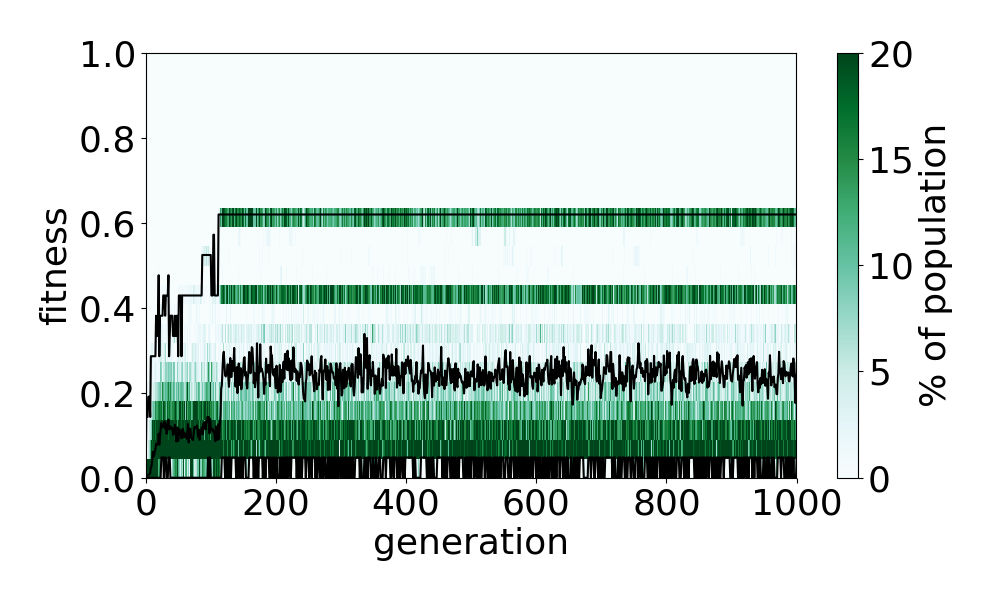
\includegraphics[width=0.3\textwidth]{img/self_adapt_2_Union_5t.png} &
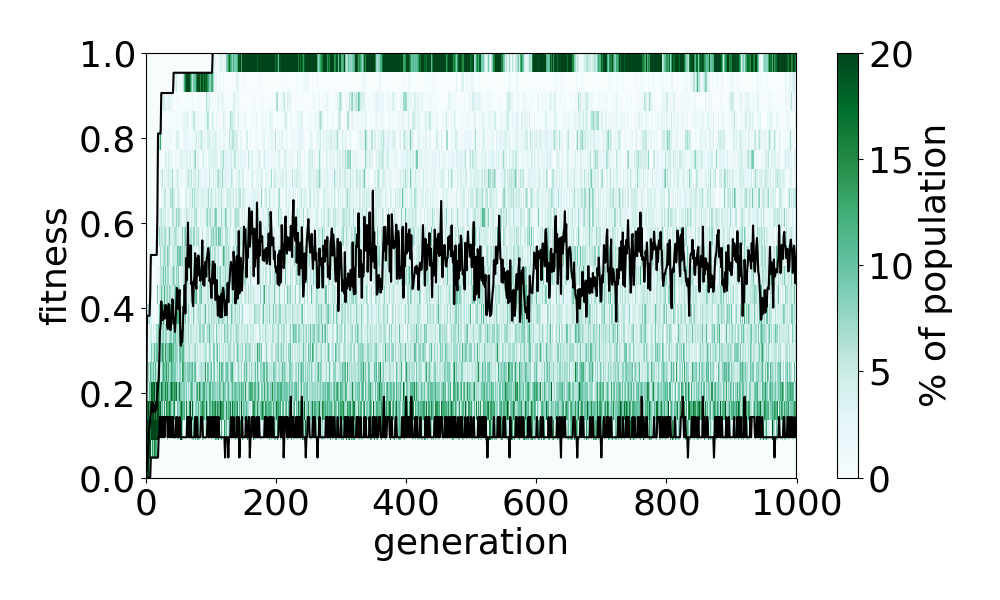
\includegraphics[width=0.3\textwidth]{img/self_adapt_2_trainer_5t.png}
\end{tabular}
\caption{Fitness density with indicated minimum, average and maximum.}
\label{fig:self_adapt_2_5t}
\end{figure}

\begin{figure}[H]
\center
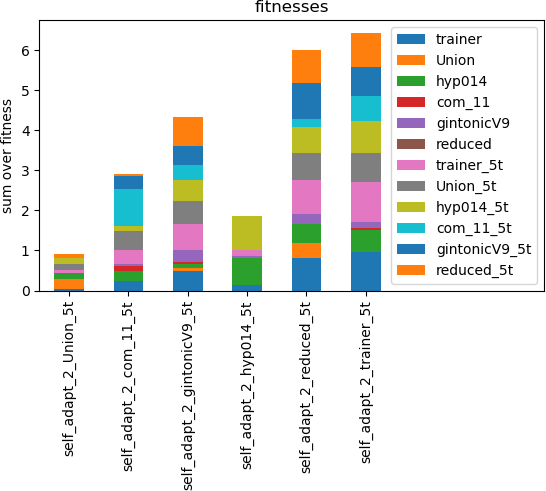
\includegraphics[width=0.4\textwidth]{img/self_adapt_2_5t.png}
\caption{trained bots against all other}
\label{fig:self_adapt_2_5t_aa}
\end{figure}

\todo{not very predictable behaviour}
\todo{works good for a few examples}
\todo{remember prof has never seen this stuff working and will be happy if it has disadvantages}

\section{Changing opponent}

200 gen \texttt{gintonicV9\_5t}, 200 gen \texttt{com\_11\_5t}, 200 gen \texttt{gintonicV9}, 200 gen \texttt{com\_11}.
\todo{argument with the previous plots that this is a good idea}
\todo{other ideas?}

\begin{figure}[H]
\center
\begin{tabular}{ccc}
standard & self adapt 1 & self adapt 2 \\
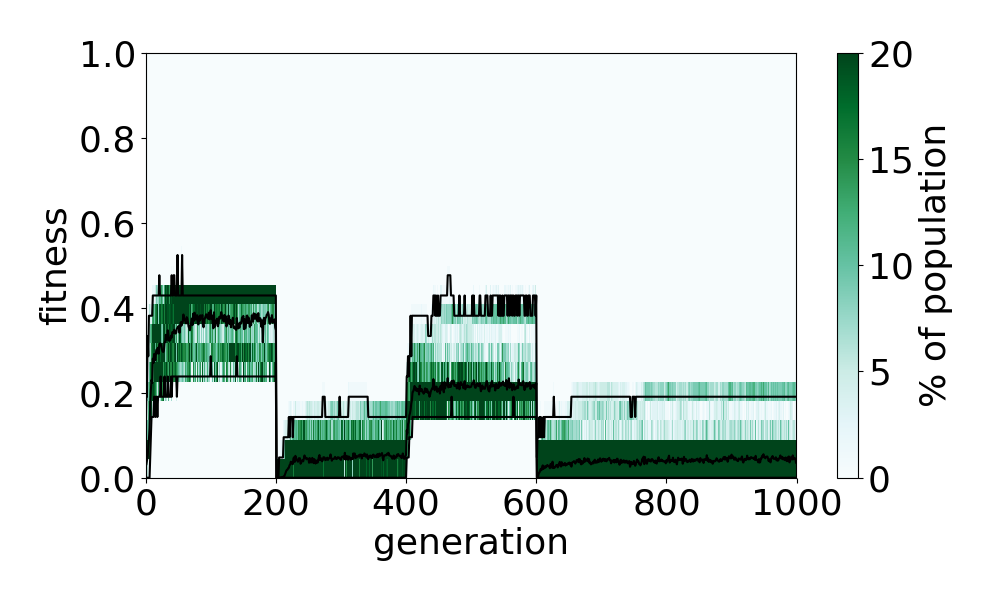
\includegraphics[width=0.3\textwidth]{img/standard_gintonicV9_5t_com_11_5t_gintonicV9_com_11.png} &
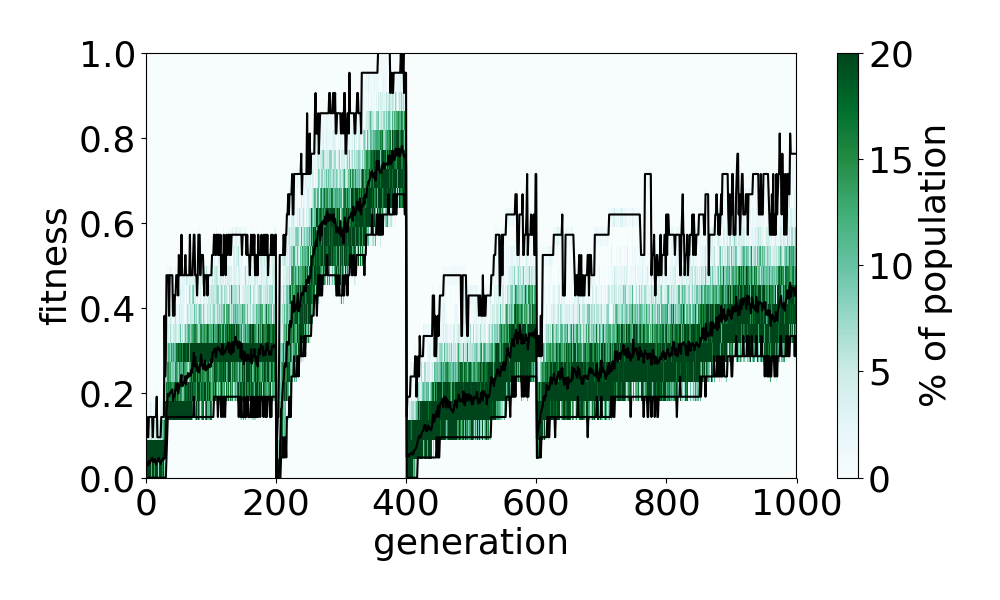
\includegraphics[width=0.3\textwidth]{img/self_adapt_1_gintonicV9_5t_com_11_5t_gintonicV9_com_11.png} &
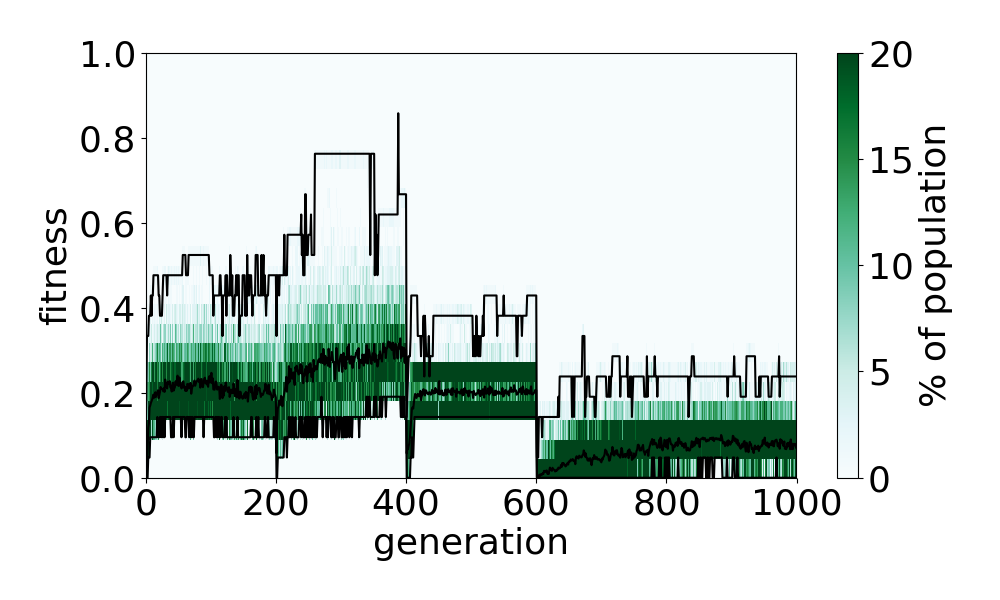
\includegraphics[width=0.3\textwidth]{img/self_adapt_2_gintonicV9_5t_com_11_5t_gintonicV9_com_11.png} \\
\end{tabular}
\caption{Fitness density with indicated minimum, average and maximum.}
\label{fig:changing opponent}
\end{figure}

\begin{figure}[H]
\center
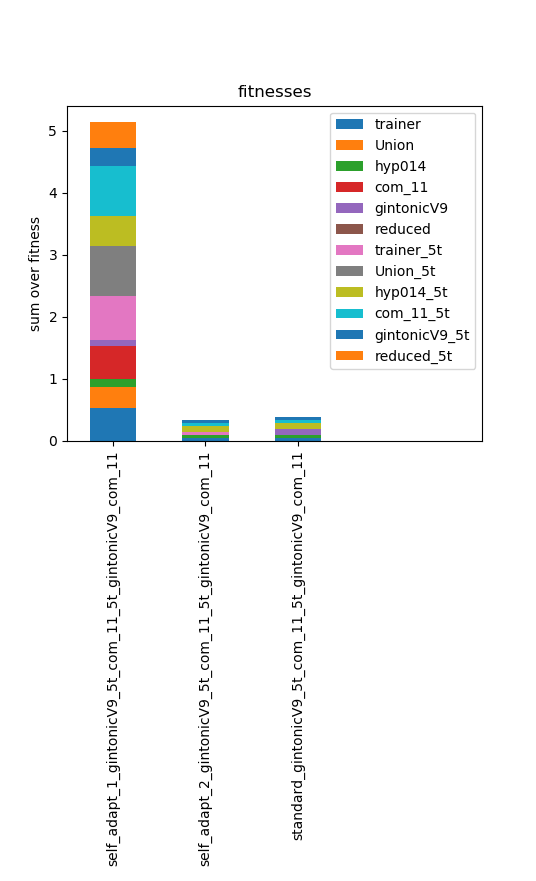
\includegraphics[width=0.4\textwidth]{img/change.png}
\caption{trained bots against all other}
\label{fig:change}
\end{figure}

\todo{only self adapt 1 works}
\todo{we could do more with more generations but loose the comparebility to the previous section}

\section{Self-training}


\subsection{last best}

\begin{figure}[H]
\center
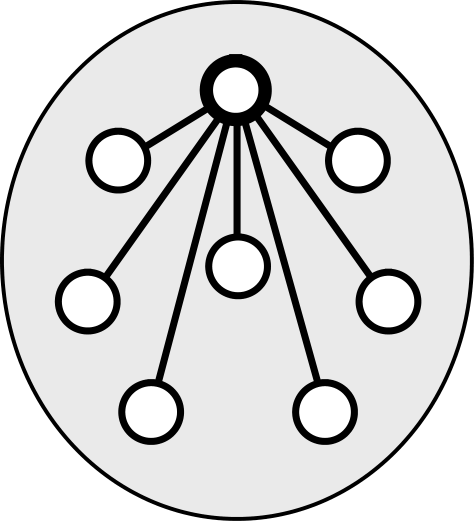
\includegraphics[width=0.155555\textwidth]{img/scheme_self_training_1.png}
\caption{Scheme for self training variant 1}
\label{fig:scheme_self_training_1}
\end{figure}

Fitness evaluated with the best bot of the last generation.

\begin{figure}[H]
\center
\begin{tabular}{cc}
standard & self adapt 1\\
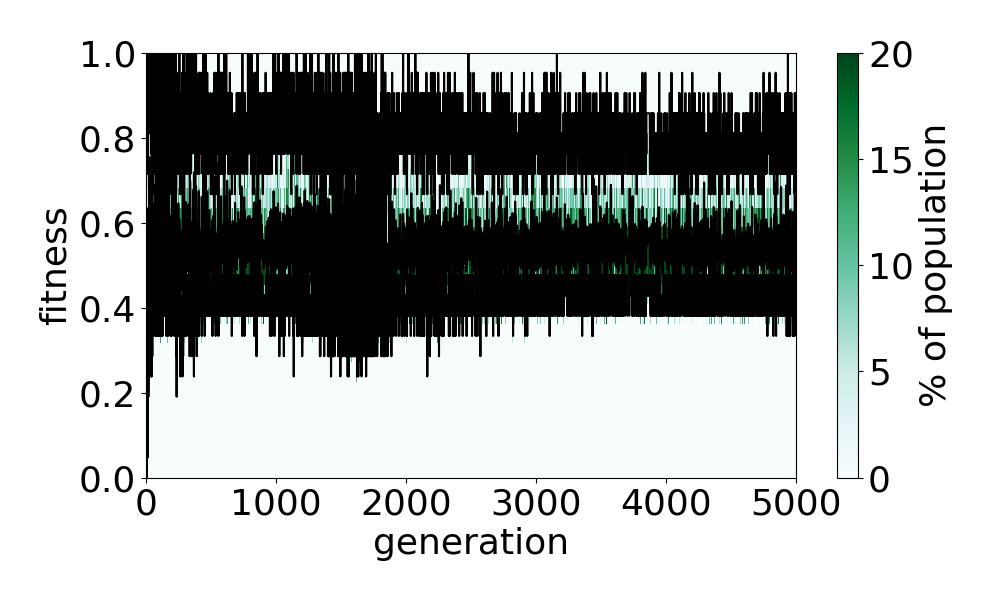
\includegraphics[width=0.3\textwidth]{img/standard_last_best.png} &
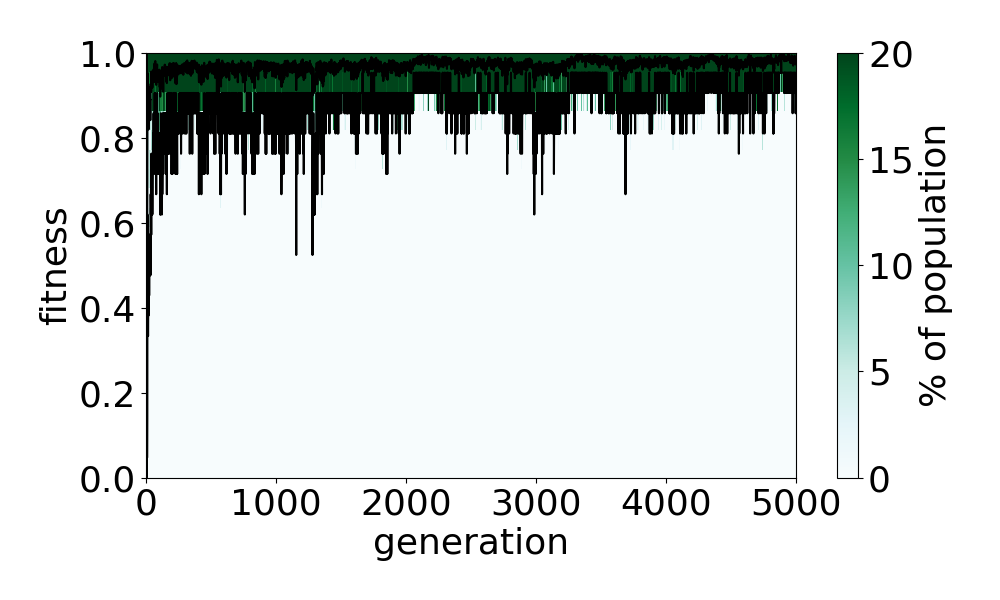
\includegraphics[width=0.3\textwidth]{img/self_adapt_1_last_best.png}
\end{tabular}
\caption{Fitness density with indicated minimum, average and maximum.}
\label{fig:last_best}
\end{figure}

\begin{figure}[H]
\center
\includegraphics[width=0.3\textwidth]{img/self_training_1.png}
\caption{trained bots against all other}
\label{fig:self_training_1}
\end{figure}

\todo{risk to end up in local optimum like self adapt 1?}


\subsection{two species}

\begin{figure}[H]
\center
\includegraphics[width=0.155555\textwidth]{img/scheme_self_training_1.png}
\caption{Scheme for self training variant 1}
\label{fig:scheme_self_training_2}
\end{figure}

\begin{figure}[H]
\center
\begin{tabular}{cc}
left side & right side \\
\includegraphics[width=0.3\textwidth]{img/standard_self_training_2_1.png} &
\includegraphics[width=0.3\textwidth]{img/standard_self_training_2_2.png} \\
\end{tabular}
\caption{Fitness density with indicated minimum, average and maximum standard mutation.}
\label{fig:standard_self_training_2}
\end{figure}

\todo{too much diversity}


\begin{figure}[H]
\center
\begin{tabular}{cc}
left side & right side \\
\includegraphics[width=0.3\textwidth]{img/self_adapt_1_self_training_2_1_oldrun.png} &
\includegraphics[width=0.3\textwidth]{img/self_adapt_1_self_training_2_2_oldrun.png}
\end{tabular}
\caption{Fitness density with indicated minimum, average and maximum with self adapt 1.}
\label{fig:self_adapt_1_self_training_2_oldrun}
\end{figure}

\todo{sadly they do not change too often}
\todo{there is still improvement even though it can not be seen in the plots because they improve themselves}

\begin{figure}[H]
\center
\begin{tabular}{cc}
left side & right side \\
\includegraphics[width=0.3\textwidth]{img/self_adapt_1_self_training_2_1.png} &
\includegraphics[width=0.3\textwidth]{img/self_adapt_1_self_training_2_2.png} \\
\end{tabular}
\caption{Fitness density with indicated minimum, average and maximum with self adapt 1 and more generations.}
\label{fig:self_adapt1_self_training_2}
\end{figure}

\begin{figure}[H]
\center
\includegraphics[width=0.4\textwidth]{img/self_training_2.png}
\caption{trained bots against all other}
\label{fig:self_training_2}
\end{figure}

\todo{we got a pretty awesome bot there which gets beaten only by reduced but never trained against it}

\section{Discussion and Future Ideas}

\todo{everything we have not done}
\todo{train the self trained bot with reduced so we maybe get a perfect score of 12}
\todo{we have not used too many inputs I still coudn't beat the bot which trained itself for four hours}
\todo{acknowledgement to the compute server}

\bibliography{refs}{}
\bibliographystyle{plain}

\end{document}
